%%%%%%%%%%%%%%%%%%%%%%%%%%%%%%%%%%%%%%%%%%%%%%
%% Compile: XeLaTeX BibTeX XeLaTeX XeLaTeX
%% Slides: Antonio Machicao y Priemer
%% Course: GK Linguistik
%%%%%%%%%%%%%%%%%%%%%%%%%%%%%%%%%%%%%%%%%%%%%%

\documentclass[a4paper,10pt, bibtotoc]{beamer}
%\documentclass[10pt,handout]{beamer}

%%%%%%%%%%%%%%%%%%%%%%%%
%%     PACKAGES      
%%%%%%%%%%%%%%%%%%%%%%%%

%%%%%%%%%%%%%%%%%%%%%%%%
%%     PACKAGES       %%
%%%%%%%%%%%%%%%%%%%%%%%%



%\usepackage[utf8]{inputenc}
%\usepackage[vietnamese, english,ngerman]{babel}   % seems incompatible with german.sty
%\usepackage[T3,T1]{fontenc} breaks xelatex

\usepackage{lmodern}
\usepackage{calligra}

\usepackage{amsmath}
\usepackage{amsfonts}
\usepackage{amssymb}
%% MnSymbol: Mathematische Klammern und Symbole (Inkompatibel mit ams-Packages!)
%% Bedeutungs- und Graphemklammern: $\lsem$ Tisch $\rsem$ $\langle TEXT \rangle$ $\llangle$ TEXT $\rrangle$ 
\usepackage{MnSymbol}
%% ulem: Strike out
\usepackage[normalem]{ulem}  

%% Special Spaces (s. Commands)
\usepackage{xspace}				
\usepackage{setspace}
%	\onehalfspacing

%% mdwlist: Special lists
\usepackage{mdwlist}	


%%%%%%%%%%%%%%%%%%%%%%%%%%%%%%%%
%% TIPA & Phonetics

\usepackage[
%noenc,
safe]{tipa}

%% TIPA Problems/Solutions:
%% Problems with U, serif fonts and ligatures

%%Test 1
%\DeclareFontSubstitution{T3}{cmss}{m}{n}

%%Test 2
%\DeclareFontSubstitution{T3}{ptm}{m}{n}

%%Test 3
%\usepackage{tipx}


%\usepackage{vowel}


%%%%%%%%%%%%%%%%%%%%%%%%%%%%%%%%
%% Examples

\usepackage{jambox}



%\usepackage{forest-v105}
%\usepackage{langsci-forest-v105-setup}


%%%%%%%%%%%%%%%%%%%%%%%%%%%%%%%%
%% Fonts for Chinese, Vietnamese, etc. (s. Graphematik)

\usepackage{xeCJK}
\setCJKmainfont{SimSun}


%\usepackage{natbib}
%\setcitestyle{notesep={:~}}


% for toggles, is loaded in hu-beamer-includes-pdflatex
%\usepackage{etex}


%%%%%%%%%%%%%%%%%%%%%%%%%%%%%%%%
%% Fonts for Fraktur

\usepackage{yfonts}

\usepackage{url}

% für UDOP
\usepackage{adjustbox}


%% huberlin: Style sheet
%\usepackage{huberlin}
\usepackage{hu-beamer-includes-pdflatex}
\huberlinlogon{0.86cm}

% %% % use this definition, if you want to see the outlines in the handout
\renewcommand{\outline}[1]{%
%\beamertemplateemptyfootbar%
\huberlinjustbarfootline
\frame{\frametitle{\outlineheading}#1}%
%\beamertemplatecopyrightfootframenumber%
\huberlinnormalfootline 
\huberlinpagedec
}



%% Last Packages
%\usepackage{hyperref}	%URLs
%\usepackage{gb4e}		%Linguistic examples

% sorry this was incompatible with gb4e and had to go.
%\usepackage{linguex-cgloss}	%Linguistic examples (patched version that works with jambox

\usepackage{multirow}  %Mehrere Zeilen in einer Tabelle
\usepackage{adjustbox} %adjusting tables
%\usepackage{array}
\usepackage{marginnote}	%Notizen




%%%%%%%%%%%%%%%%%%%%%%%%%%%%%%%%%%%%%%%%%%%%%%%%%%%%
%%%             Preamble's End                   
%%%%%%%%%%%%%%%%%%%%%%%%%%%%%%%%%%%%%%%%%%%%%%%%%%%% 

\begin{document}
	
	%%%%%%%%%%%%%%%%%%%%%%%%%%%%%%%%%%%%%%%%%%%%%%%%%%%%
%%%            MyP-Commands                     
%%%%%%%%%%%%%%%%%%%%%%%%%%%%%%%%%%%%%%%%%%%%%%%%%%%%


%%%%%%%%%%%%%%%%%%%%%%%%%%%%%%%%
% Delete Caption from Figures and Tables
\setbeamertemplate{caption}{\centering\insertcaption\par }


%%%%%%%%%%%%%%%%%%%%%%%%%%%%%%%%
% German quotation marks:
\newcommand{\gqq}[1]{\glqq{}#1\grqq{}}		%double
\newcommand{\gq}[1]{\glq{}#1\grq{}}			%simple


%%%%%%%%%%%%%%%%%%%%%%%%%%%%%%%%
% Abbreviations in German
% package needed: xspace
% Short space in German abbreviations: \,	
\newcommand{\idR}{\mbox{i.\,d.\,R.}\xspace}
\newcommand{\su}{\mbox{s.\,u.}\xspace}
%\newcommand{\ua}{\mbox{u.\,a.}\xspace}       % in abbrev
\newcommand{\vgl}{\mbox{vgl.}\xspace}       % in abbrev
%\newcommand{\zB}{\mbox{z.\,B.}\xspace}       % in abbrev
%\newcommand{\s}{s.~}
%not possibel: \dh --> d.\,h.

%rot unterstrichen
%\newcommand{\rotul}[1]{\textcolor{red}{\underline{#1}}}

%%%%%%%%%%%%%%%%%%%%%%%%%%%%%%%%
%Abbreviations in English
\newcommand{\ao}{a.o.\ }	% among others
%\newcommand{\cf}[1]{(cf.~#1)}	% confer = compare
\renewcommand{\ia}{i.a.}	% inter alia = among others
%\newcommand{\ie}{i.e.~}	% id est = that is
\newcommand{\fe}{e.g.~}	% exempli gratia = for example
%not possible: \eg --> e.g.~
\newcommand{\vs}{vs.\ }	% versus
\newcommand{\wrt}{w.r.t.\ }	% with respect to


%%%%%%%%%%%%%%%%%%%%%%%%%%%%%%%%
% Dash:
\newcommand{\gs}[1]{--\,#1\,--}


%%%%%%%%%%%%%%%%%%%%%%%%%%%%%%%%
% Rightarrow with and without space
\def\ra{\ensuremath\rightarrow}			%without space
\def\ras{\ensuremath\rightarrow\ }		%with space


%%%%%%%%%%%%%%%%%%%%%%%%%%%%%%%%
%% X-bar notation

%% Notation with primes (not emphasized): \xbar{X}
\newcommand{\MyPxbar}[1]{#1$^{\prime}$}
\newcommand{\xxbar}[1]{#1$^{\prime\prime}$}
\newcommand{\xxxbar}[1]{#1$^{\prime\prime\prime}$}

%% Notation with primes (emphasized): \exbar{X}
\newcommand{\exbar}[1]{\emph{#1}$^{\prime}$}
\newcommand{\exxbar}[1]{\emph{#1}$^{\prime\prime}$}
\newcommand{\exxxbar}[1]{\emph{#1}$^{\prime\prime\prime}$}

% Notation with zero and max (not emphasized): \xbar{X}
\newcommand{\zerobar}[1]{#1$^{0}$}
\newcommand{\maxbar}[1]{#1$^{\textsc{max}}$}

% Notation with zero and max (emphasized): \xbar{X}
\newcommand{\ezerobar}[1]{\emph{#1}$^{0}$}
\newcommand{\emaxbar}[1]{\emph{#1}$^{\textsc{max}}$}

%% Notation with bars (already implemented in gb4e):
% \obar{X}, \ibar{X}, \iibar{X}, \mbar{X} %Problems with \mbar!
%
%% Without gb4e:
\newcommand{\overbar}[1]{\mkern 1.5mu\overline{\mkern-1.5mu#1\mkern-1.5mu}\mkern 1.5mu}
%
%% OR:
\newcommand{\MyPibar}[1]{$\overline{\textrm{#1}}$}
\newcommand{\MyPiibar}[1]{$\overline{\overline{\textrm{#1}}}$}
%% (emphasized):
\newcommand{\eibar}[1]{$\overline{#1}$}
\newcommand{\eiibar}[1]{\overline{$\overline{#1}}$}

%%%%%%%%%%%%%%%%%%%%%%%%%%%%%%%%
%% Subscript & Superscript: no italics
\newcommand{\MyPdown}[1]{\textsubscript{#1}}
\newcommand{\MyPup}[1]{\textsuperscript{#1}}

%%%%%%%%%%%%%%%%%%%%%%%%%%%%%%%%
%% Small caps subscripts & superscripts
\newcommand{\scdown}[1]{\textsubscript{\textsc{#1}}}
\newcommand{\scup}[1]{\textsuperscript{\textsc{#1}}}

%%%%%%%%%%%%%%%%%%%%%%%%%%%%%%%%
% Objekt language marking:
%\newcommand{\obj}[1]{\glqq{}#1\grqq{}}	%German double quotes
%\newcommand{\obj}[1]{``#1''}			%English double quotes
%\newcommand{\MyPobj}[1]{\emph{#1}}		%Emphasising
\newcommand{\MyPobj}[1]{\textit{#1}}		%Emphasising

%%%%%%%%%%%%%%%%%%%%%%%%%%%%%%%%
% Size:
\newcommand{\size}[1]{#1}	% f.e. resize citations


%%%%%%%%%%%%%%%%%%%%%%%%%%%%%%%%
%% Semantic types (<e,t>), features, variables and graphemes in angled brackets 

%%% types and variables, in math mode: angled brackets + italics + no space
%\newcommand{\type}[1]{$<#1>$}

%%% OR more correctly: 
%%% types and variables, in math mode: chevrons! + italics + no space
\newcommand{\MyPtype}[1]{$\langle #1 \rangle$}

%%% features and graphemes, in math mode: chevrons! + italics + no space
\newcommand{\abe}[1]{$\langle #1 \rangle$}


%%% features and graphemes, in math mode: chevrons! + no italics + space
\newcommand{\ab}[1]{$\langle$#1$\rangle$}  %%same as \abu  
\newcommand{\abu}[1]{$\langle$#1$\rangle$} %%Umlaute


%% Presuppositions
\newcommand{\prspp}{$\gg$} 

%% Implicature
\newcommand{\implc}{$+ \mkern-5mu >$} 

%% Enttailment
\newcommand{\ent}{$\vDash$}

%% Other semantic symbols: 
%% entailment: $\Rightarrow$ $\vDash$
%% equivalence: $\Leftrightarrow$ $\equiv$
%% biconditional: $\leftrightarrow$ 
%% lexical rule: $\mapsto$
%% greater/less/equal: $>$ $\geq$ $<$ $\leq$
%% definition: $:=$ $=$\textsubscript{def}


%%%%%%%%%%%%%%%%%%%%%%%%%%%%%%%%
% Marking text with colour:
% package needed: xcolor
% Command \alert{} in Beamer >> FU-grün (leider!! @Stefan)

%%%neue Farbbefehle in Anlehnung an rotul
%%%(s. hu-beamer-includes-pdflatex.sty in texmf)

%% Farbdefinitionen:

\definecolor{HUred}{RGB}{138,15,20}
\definecolor{HUblue}{RGB}{0,55,108}
\definecolor{HUgreen}{RGB}{0,87,44}

%\newcommand{\alertred}[1]{\textcolor{red}{#1}}  % basic red
\newcommand<>{\alertred}[1]{{\color#2[RGB]{138,15,20}#1}}  %HU rot + overlay

%\newcommand{\alertblue}[1]{\textcolor{blue}{#1}} 		% basic blue
\newcommand<>{\alertblue}[1]{{\color#2[RGB]{0,55,108}#1}} %HU blue + overlay

%\newcommand{\alertgreen}[1]{\textcolor{green}{#1}}	% basic green
\newcommand<>{\alertgreen}[1]{{\color#2[RGB]{0,87,44}#1}} %HU green + overlay


%%% Verwendung der oben definierten Farben mit Unterschied in Handout und Beamer:

\mode<handout>{%
	\newcommand<>{\hured}[1]{\only#2{\underline{#1}}}
	\newcommand<>{\hublue}[1]{\only#2{\textbf{#1}}}
	\newcommand<>{\hugreen}[1]{\only#2{\textsc{#1}}}
}
%
\mode<beamer>{%
	\newcommand<>{\hured}[1]{\alertred#2{#1}}
	\newcommand<>{\hublue}[1]{\alertblue#2{#1}}
	\newcommand<>{\hugreen}[1]{\alertgreen#2{#1}}
}


%%%%%%%%%%%%%%%%%%%%%%%%%%%%%%%%
%% Outputbox
\newcommand{\outputbox}[1]{\noindent\fbox{\parbox[t][][t]{0.98\linewidth}{#1}}\vspace{0.5em}}


%%%%%%%%%%%%%%%%%%%%%%%%%%%%%%%%
%% (Syntactic) Trees
% package needed: forest
%
%% Setting for simple trees
\forestset{
	MyP edges/.style={for tree={parent anchor=south, child anchor=north}}
}

%% this is taken from langsci-setup file
%% Setting for complex trees
%% \forestset{
%% 	sm edges/.style={for tree={parent anchor=south, child anchor=north,align=center}}, 
%% background tree/.style={for tree={text opacity=0.2,draw opacity=0.2,edge={draw opacity=0.2}}}
%% }

\newcommand\HideWd[1]{%
	\makebox[0pt]{#1}%
}

%%%%%%%%%%%%%%%%%%%%%%%%%%%%%%%
%%solutions in green + w/ jambox
\newcommand{\loesung}[2]{\jambox{\visible<#1->{\alertgreen{#2}}}}

%%%%%%%%%%%%%%%%%%%%%%%%%%%%%%%%
%% TIPA Lösungen           

%%Tipa serif font fixed (requires package 'Linux Libertine B')

%% Solution 1 (RF)
%% Tipa font:
%\renewcommand\textipa[1]{{\fontfamily{cmr}\tipaencoding #1}}

%% Solution 2 (RF): older code for texlive 2017?
%\newfontfamily{\tipacm}[Scale=MatchUppercase]{Linux Libertine B}
%\renewcommand\useTIPAfont{\tipacm}

%\NewEnviron{IPA}{\expandafter\textipa\expandafter{\BODY}} %% not needed anymore

%% Solution 3 (RF): this solution is working but with problems with ligatures
%%% works for texlive 2018
\newfontfamily{\ipafont}[Scale=MatchUppercase]{Linux Libertine B}
\def\useTIPAfont{\ipafont}

%% Solution 4 (Kopecky & MyP): Test package: tipx (s. localpackages) and comment "Solution 3" 


%%%%%%%%%%%%%%%%%%%%%%%%%%%%%%%%
%% Toggles                  


\newtoggle{uebung}
\newtoggle{loesung}\togglefalse{loesung}

\newtoggle{hausaufgabe}

%\newtoggle{ha-loesung}\togglefalse{ha-loesung}
\newtoggle{phonologie-loesung}
\newtoggle{graphematik-loesung}


%% Neue Toggle-Struktur
\newtoggle{toc}
\newtoggle{sectoc}
\newtoggle{gliederung}

\newtoggle{ue-loesung}
\newtoggle{ha-loesung}
%%

% The toc is not needed on Handouts. Save trees.
\mode<handout>{
\togglefalse{toc}
}

\newtoggle{hpsgvorlesung}\togglefalse{hpsgvorlesung}
\newtoggle{syntaxvorlesungen}\togglefalse{syntaxvorlesungen}

%\includecomment{psgbegriffe}
%\excludecomment{konstituentenprobleme}
%\includecomment{konstituentenprobleme-hinweis}

\newtoggle{konstituentenprobleme}\togglefalse{konstituentenprobleme}
\newtoggle{konstituentenprobleme-hinweis}\toggletrue{konstituentenprobleme-hinweis}

%\includecomment{einfsprachwiss-include}
%\excludecomment{einfsprachwiss-exclude}
\newtoggle{einfsprachwiss-include}\toggletrue{einfsprachwiss-include}
\newtoggle{einfsprachwiss-exclude}\togglefalse{einfsprachwiss-exclude}

\newtoggle{psgbegriffe}\toggletrue{psgbegriffe}

\newtoggle{gb-intro}\togglefalse{gb-intro}


%%%%%%%%%%%%%%%%%%%%%%%%%%%%%%%%
%% Useful commands                    

%%%%%%%%%%%%%%%%%%%%%
%% FOR ITEMS:
%\begin{itemize}
%  \item<2-> from point 2
%  \item<3-> from point 3 
%  \item<4-> from point 4 
%\end{itemize}
%
% or: \onslide<2->
% or \only<2->{Text}
% or: \pause

%%%%%%%%%%%%%%%%%%%%%
%% VERTICAL SPACE:
% \vspace{.5cm}
% \vfill

%%%%%%%%%%%%%%%%%%%%%
% RED MARKING OF TEXT:
%\alert{bis spätestens Mittwoch, 18 Uhr}
%\newcommand{\alertred}[1]{\textcolor{red}{#1}}

%%%%%%%%%%%%%%%%%%%%%
%% RESCALE BIG TABLES:
%\scalebox{0.8}{
%For Big Tables
%}

%%%%%%%%%%%%%%%%%%%%%
%% BLOCKS:
%\begin{alertblock}{Title}
%Text
%\end{alertblock}
%
%\begin{block}{Title}
%Text
%\end{block}
%
%\begin{exampleblock}{Title}
%Text
%\end{exampleblock}

%%%%%%%%%%%%%%%%%%%%%
%% JAMBOX FOR EXAMPLES:
%\ea 
%\settowidth\jamwidth{Test} 
%Die Studierenden, die weitgehend von Stipendien leben, erhalten einen Mietzuschuss. 
%\jambox{Test}
%\z 

%%%%%%%%%%%%%%%%%%%%%
%% TOGGLES:


%%%%%%%%%%%%%%%%%%%%%%%%%%%%%%%%%%
%%%%%%%%%%%%%%%%%%%%%%%%%%%%%%%%%%
%\subsection{Übung}
%
%%%%%%%%%%%%%%%%%%%%%%%%%%%%%%%%%%
%%%%%%%%%%%%%%%%%%%%%%%%%%%%%%%%%%
%\iftoggle{uebung}{
%%%%%%%%%%%%%%%%%%%%%%%%%%%%%%%%%%
%\begin{frame}
%\frametitle{Übung}
%
%\end{frame}
%
%} 
%%% END true = Q
%%% BEGIN false = Q + A
%{
%%%%%%%%%%%%%%%%%%%%%%%%%%%%%%%%%%
%\begin{frame}
%\frametitle{Übung}
%
%\end{frame}
%%%%%%%%%%%%%%%%%%%%%%%%%%%%%%%%%%
%
%\begin{frame}
%\frametitle{Lösung}
%
%\end{frame}
%
%}%% END LOESUNG	
%%%%%%%%%%%%%%%%%%%%%%%%%%%%%%%%%%


%%%%%%%%%%%%%%%%%%%%%%%%%%%%%%%%%%
%%%%%%%%%%%%%%%%%%%%%%%%%%%%%%%%%%
%\subsection{Hausaufgabe}
%
%%%%%%%%%%%%%%%%%%%%%%%%%%%%%%%%%%
%%%%%%%%%%%%%%%%%%%%%%%%%%%%%%%%%%
%\iftoggle{hausaufgabe}{
%%%%%%%%%%%%%%%%%%%%%%%%%%%%%%%%%%
%
%\begin{frame}
%\frametitle{Hausaufgabe}
%
%\end{frame}
%
%} 
%%% END true = Q
%%% BEGIN false = Q + A
%{
%%%%%%%%%%%%%%%%%%%%%%%%%%%%%%%%%%
%
%\begin{frame}
%\frametitle{Hausaufgabe}
%
%\end{frame}
%
%
%%%%%%%%%%%%%%%%%%%%%%%%%%%%%%%%%%
%%%%%%%%%%%%%%%%%%%%%%%%%%%%%%%%%%
%\subsection*{Lösung der Hausaufgabe}
%
%%%%%%%%%%%%%%%%%%%%%%%%%%%%%%%%%%
%
%\begin{frame}
%\frametitle{Lösung}
%
%\end{frame}
%
%}%% END LOESUNG	
%%%%%%%%%%%%%%%%%%%%%%%%%%%%%%%%%%

	
	%%%% ue-loesung
	%%%% true: Übung & Lösungen (slides) / false: nur Übung (handout)
	\toggletrue{ue-loesung}
	
	%%%% ha-loesung
	%%%% true: Hausaufgabe & Lösungen (slides) / false: nur Hausaufgabe (handout)
	\toggletrue{ha-loesung}
	
	%%%% toc
	%%%% true: TOC am Anfang von Slides / false: keine TOC am Anfang von Slides
	\toggletrue{toc}
	
	%%%% sectoc
	%%%% true: TOC für Sections / false: keine TOC für Sections (StM handout)
	\toggletrue{sectoc}
	
	%%%% gliederung
	%%%% true: Gliederung für Sections / false: keine Gliederung für Sections
	%	\toggletrue{gliederung}
	
	
	%%%%%%%%%%%%%%%%%%%%%%%%%%%%%%%%%%%%%%%%%%%%%%%%
%% Compile the master file!
%% 		Slides: Antonio Machicao y Priemer
%% 		Course: GK Linguistik
%%%%%%%%%%%%%%%%%%%%%%%%%%%%%%%%%%%%%%%%%%%%%%%%


%%%%%%%%%%%%%%%%%%%%%%%%%%%%%%%%%%%%%%%%%%%%%%%%%%%%
%%%             Metadata                         
%%%%%%%%%%%%%%%%%%%%%%%%%%%%%%%%%%%%%%%%%%%%%%%%%%%%      

\title{Grundkurs Linguistik}

\subtitle{Semantik II \& Pragmatik I}

\author[A. Machicao y Priemer]{
	{\small Antonio Machicao y Priemer}
	\\
	{\footnotesize \url{http://www.linguistik.hu-berlin.de/staff/amyp}}
	%	\\
	%	\href{mailto:mapriema@hu-berlin.de}{mapriema@hu-berlin.de}}
}

\institute{Institut für deutsche Sprache und Linguistik}

\date{ }

%\publishers{\textbf{6. linguistischer Methodenworkshop \\ Humboldt-Universität zu Berlin}}

%\hyphenation{nobreak}


%%%%%%%%%%%%%%%%%%%%%%%%%%%%%%%%%%%%%%%%%%%%%%%%%%%%
%%%             Preamble's End                   
%%%%%%%%%%%%%%%%%%%%%%%%%%%%%%%%%%%%%%%%%%%%%%%%%%%%      


%%%%%%%%%%%%%%%%%%%%%%%%%    
\huberlintitlepage[22pt]
\iftoggle{toc}{
\frame{
\begin{multicols}{2}
	\frametitle{Inhaltsverzeichnis}\tableofcontents
	%[pausesections]
\end{multicols}
}
}


%%%%%%%%%%%%%%%%%%%%%%%%%%%%%%%%%%
%%%%%%%%%%%%%%%%%%%%%%%%%%%%%%%%%%
%%%%%LITERATURE:

\nocite{Brandt&Co06a} 
\nocite{Glueck05a} 
\nocite{Grewendorf&Co91a} 
\nocite{Luedeling2009a} 

%% Allgemein
\nocite{Glueck&Roedel16a}
\nocite{Luedeling2009a}
\nocite{Meibauer&Co07a} 
\nocite{Repp&Co15a} 

%% Morphologie
%\nocite{Eisenberg04}

%% Syntax
%\nocite{Adger04a}
%\nocite{Altmann&Hofmann08a} % Satztypen & Satzmodi
%\nocite{Altmann93a} % Satztypen & Satzmodi
%\nocite{Brandt&Co06a} 
%\nocite{Fanselow&Sascha87a}
%\nocite{Fanselow&Sascha93a}
%\nocite{Fries&MyP16b} % Akzeptabilität
%\nocite{Fries16a} % Grammatikalität
%\nocite{Fries&MyP16d} % Kompetenz vs Performanz
%\nocite{Fries&MyP16c} % GG
%\nocite{Fries&MyP16a} % X-Bar-Theorie
%\nocite{Fries16e} % Satztyp
%\nocite{Fries16d} % Satzmodus 
\nocite{Grewendorf&Co91a} 
%\nocite{MyP17b} % Kerngrammatik
%\nocite{MyP18a} % Konstituententest
%\nocite{MyP18b} % Kopf
%\nocite{MyP18c} % Phrase
%\nocite{MyP18s} % Funktionale Kategorie
%\nocite{MyP18t} % Argumentstruktur
%\nocite{MuellerS13f} 
%\nocite{MuellerS15b}
%\nocite{Stechow&Sternefeld88a}
%\nocite{Sternefeld06a}
%\nocite{Sternefeld06b}
%\nocite{Woellstein10a} % Topologisches Feldermodell

%% Semantik & Pragmatik
\nocite{Loebner15a} %% Semantics
\nocite{Loebner15b} %% Semantics
\nocite{Lohnstein11} %% Semantics
%\nocite{MyP16a} %% Bikonditional
\nocite{Partee&Co93a} %% Semantics
\nocite{ZimmermannT&Sternefeld13a} %% Semantics


%%%%%%%%%%%%%%%%%%%%%%%%%%%%%%%%%%%
\section{Pragmatik}
%%%%%%%%%%%%%%%%%%%%%%%%%%%%%%%%%%

\begin{frame}
\frametitle{Begleitlektüre}

\begin{itemize}
	
	\item \textbf{obligatorisch:}
		\begin{itemize}
		\item AM S.~107--116
		\end{itemize}
	
	\item \textbf{optional:}
		\begin{itemize}
		\item \citet{Meibauer&Co07a}: Kapitel 6 (S.~210--240)
		\end{itemize}

\end{itemize}	

\end{frame}


%%%%%%%%%%%%%%%%%%%%%%%%%%%%%%%%%%%
%%%%%%%%%%%%%%%%%%%%%%%%%%%%%%%%%%%
%
\subsection{Einführung}

%% MyP: Contents
\iftoggle{sectoc}{
	\frame{
		%\begin{multicols}{2}
		\frametitle{~}
		\tableofcontents[currentsubsection,subsubsectionstyle=hide]
		%\end{multicols}
	}
}
%%%%%%%%%%%%%%%%%%%%%%%%%%%%%%%%%%%%%

\begin{frame}
\frametitle{Einführung}

\begin{itemize}
	\item Pragmatik: jüngste sprachwissenschaftliche Disziplin
	\item Schnittstellen zur Philosophie, Soziologie, Psychologie
	\item Gegenstand: \textbf{Gebrauch} sprachlicher Ausdrücke in einer bestimmten Situation (Kontext)
	\medskip
	\item Semantik \vs Pragmatik (grob):
	
	\begin{itemize}
		\item Semantik:\\
kontextunabhängige (und durch Wahrheitsbedingungen erfassbare) Bedeutung
		\item Pragmatik: \\
kontextabhängige  (und durch Wahrheitsbedingungen nicht erfassbare) Bedeutung
	\end{itemize}
	
\end{itemize}

\end{frame}


%%%%%%%%%%%%%%%%%%%%%%%%%%%%%%%%%%%%%%%

\begin{frame}
\frametitle{Einführung}

\begin{itemize}
	\item Semantik: Bedeutung aus Wörtern $+$ Strukturen
	\medskip
	\item Pragmatik: kontextuell relevante Interpretation
	
	\begin{itemize}
		\item Ich habe zwei Flaschen Wein.
		
		\begin{itemize}
			\item Semantik: Der Sprecher besitzt zwei Flaschen, die mit Wein gefüllt sind.
			\item Pragmatik: Der Sprecher besitzt nicht mehr als zwei Flaschen. (Nutzung: Zollerklärung, Angebot, Mitteilung, \dots)
		\end{itemize}
	\end{itemize}
\end{itemize}

\end{frame}


%%%%%%%%%%%%%%%%%%%%%%%%%%%%%%%%%%%%%%%
%%%%%%%%%%%%%%%%%%%%%%%%%%%%%%%%%%%%%%
%
\subsection{Kontext}
%
%%%%%%%%%%%%%%%%%%%%%%%%%%%%%%%%%%%%%%%%
%% MyP: Contents
\iftoggle{sectoc}{
	\frame{
		%\begin{multicols}{2}
		\frametitle{~}
		\tableofcontents[currentsubsection,subsubsectionstyle=hide]
		%\end{multicols}
	}
}
%%%%%%%%%%%%%%%%%%%%%%%%%%%%%%%%%%%%%

\begin{frame}
\frametitle{Kontext}

\begin{itemize}
	\item Kontextuell relevante Aspekte von Bedeutung:
	
\vspace{5mm}
	
	\begin{itemize}
		\item \textbf{Äu\ss{}erungssituation} \\
Zeitpunkt, Sprecher, Hörer, \dots
		\medskip
		
		\item \textbf{Sprachlicher Kontext}\\
Vorhergehende Äu\ss{}erungen, Diskurs-Thema, \dots
		\medskip
		
		\item \textbf{Informationeller Kontext} \\
Was wei\ss{} der Sprecher, was nimmt der Sprecher über den Hörer an, Weltwissen, \dots
		\medskip
		
		\item \textbf{Intentionaler Kontext} \\
Was sind die Ziele/""Wünsche/""Pläne des Sprechers?
	\end{itemize}
	
\end{itemize}

\end{frame}


%%%%%%%%%%%%%%%%%%%%%%%%%%%%%%%%%%%%%%%%%%%%%
%%%%%%%%%%%%%%%%%%%%%%%%%%%%%%%%%%%%%%%%%%%%%%
%
\subsubsection{Deixis}
%
%%%%%%%%%%%%%%%%%%%%%%%%%%%%%%%%%%%%%%%%%%%%
%\iftoggle{sectoc}{
%\frame{
%\frametitle{~}
%	\tableofcontents[currentsubsection,subsubsectionstyle=hide]
%}
%}
%%%%%%%%%%%%%%%%%%%%%%%%%%%%%%%%%%%%%%%%%%%%

\begin{frame}
\frametitle{Deixis}

\begin{itemize}
	\item Deixis: Vorgang des Zeigens
\end{itemize}

	\begin{block}{Deiktische Ausdrücke}
	\textbf{Deiktische} (oder indexikalische) \textbf{Ausdrücke} bezeichnen sprachliche Ausdrücke, die sich auf die Aspekte der Äu\ss{}erungssituation beziehen (Person-, Raum- und Zeitstruktur).
	\end{block}

\begin{itemize}

		\item Referenz: Aspekte der Äu\ss{}erungssituation
		\medskip
		\item Referenz von deiktischen Ausdrücken ist anders als bei referierenden Ausdrücken.
\end{itemize}

\end{frame}


%%%%%%%%%%%%%%%%%%%%%%%%%%%%%%%%%%%%%%%

\begin{frame}
\frametitle{Deixis}

\begin{columns}

\begin{column}[t]{0.5\textwidth}		
\begin{itemize}
	\item \textbf{Personaldeixis} 
	
	\begin{itemize}
		\item Aktuelle Gesprächsrollen
		\item Sprecher/Adressat: \emph{ich, du, wir, \dots}
	\end{itemize}
	
	\item \textbf{Sozialdeixis}
	
	\begin{itemize}
		\item Distanzform für Adressaten: \emph{Sie} (\vs \emph{du})
	\end{itemize}
	
	\item \textbf{Objektdeixis}
	
	\begin{itemize}
		\item Situativ-deiktisch verwendete Pronomina
		\item Referenz auf 3. Pers./Obj.: \emph{dieser, jener, der, er, \dots}
	\end{itemize}
	
\end{itemize}
\end{column}
	
\begin{column}[t]{0.5\textwidth}
	\begin{itemize}
			\item \textbf{Lokaldeixis}
				
		\begin{itemize}
			\item Referenz auf Ort: \emph{hier, dort, \dots}
		\end{itemize}
			
		\item \textbf{Temporaldeixis}
				
		\begin{itemize}
			\item Referenz auf Zeit: \emph{gestern, heute, \dots}
		\end{itemize}
				
			\end{itemize}
\end{column}
	
\end{columns}

\end{frame}


%%%%%%%%%%%%%%%%%%%%%%%%%%%%%%%%%%%%%
%%%%%%%%%%%%%%%%%%%%%%%%%%%%%%%%%%%%%
%
\subsubsection{Anaphorik}
%
%%%%%%%%%%%%%%%%%%%%%%%%%%%%%%%%%%%%%%
%\iftoggle{sectoc}{
%	\begin{frame
%\frametitle{~}
%	\tableofcontents[currentsubsection,subsubsectionstyle=hide]
%}
%}
%%%%%%%%%%%%%%%%%%%%%%%%%%%%%%%%%%%%%%%

\begin{frame}
\frametitle{Anaphorik}

\begin{block}{Anaphorische Ausdrücke (Anapher)}
	Sprachliche Ausdrücke, die sich auf sprachliche Einheiten im vorhergehenden sprachlichen Kontext beziehen.
\end{block}

\begin{itemize}
	\item Anaphorik \vs Deixis \ras Art des Kontextes
	\medskip
	\item \textbf{Textdeixis}
	
	\eal 
	\ex Peter hat \alertred{sich} rasiert.
	\ex Die Hausaufgabe war so einfach, dass alle \alertred{sie} sehr schnell lösen konnten.
	\zl
	
\end{itemize}
	
\end{frame}


%%%%%%%%%%%%%%%%%%%%%%%%%%%%%%%%%%%%%%%

\begin{frame}
\frametitle{Anaphorik}

\begin{block}{Koreferenz}
	Bezug zweier (oder mehrerer) Ausdrücke auf den gleichen Referenten in einem Text (oder Satz).
\end{block}

\begin{block}{Antezedens}
	Erstgenannter referentieller Ausdruck in einer anaphorischen Kette.
\end{block}


	
		\eal 
		\ex \alertred{Peter} hat sich rasiert. (Syntaktische Anapher $=$ Reflexivpron.)
		\ex \alertred{Die Hausaufgabe} war so einfach, dass alle sie sehr schnell lösen konnten.
		\zl
		
		\begin{itemize}
			\item Antezedens: \gqq{Peter} von \gqq{sich} und \gqq{die Hausaufgabe} von \gqq{sie}
		\end{itemize}
	


\end{frame}


%%%%%%%%%%%%%%%%%%%%%%%%%%%%%%%%%%%%%%%

\begin{frame}
\frametitle{Anaphorik}

%\begin{itemize}
%	\item \textbf{Anapher}
	\begin{block}{Anapher}
		\ea Wie viel an \textbf{Grice} auch immer auszusetzen ist, selbst die schärfsten Kritiker sehen \textbf{ihn} als einen der wichtigsten Pragmatiker an.
		\z
	\end{block}
	
%	\item \textbf{Katapher}

	\begin{block}{Katapher}
		\ea Wie viel an \textbf{ihm} auch immer auszusetzen ist, selbst die schärfsten Kritiker sehen \textbf{Grice} als einen der wichtigsten Pragmatiker an.
		\z
	\end{block}
	
%\end{itemize}

\end{frame}


%%%%%%%%%%%%%%%%%%%%%%%%%%%%%%%%%%%%%%%
%%%%%%%%%%%%%%%%%%%%%%%%%%%%%%%%%%%%%%
%
\subsubsection{Übung}
%
%%%%%%%%%%%%%%%%%%%%%%%%%%%%%%%%%%%%%%%%
%%%%%%%%%%%%%%%%%%%%%%%%%%%%%%%%%%%%%%%
%\iftoggle{sectoc}{
%\begin{frame
%\frametitle{~}
%	\tableofcontents[currentsubsection,subsubsectionstyle=hide]
%}
%}
%%%%%%%%%%%%%%%%%%%%%%%%%%%%%%%%%%%%%%%

\begin{frame}
\frametitle{Übung}

%\begin{itemize}
%	\item 
	Markieren und bestimmen Sie die deiktischen und anaphorischen Ausdrücke.
	
%	\begin{enumerate}
	\ea \label{ex:08ue8} Morgen werde ich sie besuchen, obwohl es mir zeitlich nicht passt.
	\ex \label{ex:08ue9} Gestern regnete es vor dem Supermarkt.
	\ex \label{ex:08ue10}Am 10.02.2014 hat Peter einen Sack Kartoffeln gekauft.
	\ex \label{ex:08ue11}Ich treffe Sie in Ihrem Büro.
	\ex \label{ex:08ue12}Der Dozent wei\ss{}, dass es gut für Sie ist, das zu lernen.
	\ex \label{ex:08ue13}Karl hat nicht hingeschaut und dann hat er mich angefahren.
	\ex \label{ex:08ue14}Mario hat ihn rasiert und Peter hat sich gewaschen.
	\z
%	\end{enumerate}
	
%\end{itemize}

\end{frame}


%%%%%%%%%%%%%%%%%%%%%%%%%%%%%%%%%%%%%%%

\iftoggle{ue-loesung}{
	
	%%%%%%%%%%%%%%%%%%%%%%%%%%%%%%%%%%
%% UE 1 - 08 Pragmatik
%%%%%%%%%%%%%%%%%%%%%%%%%%%%%%%%%%

\begin{frame}
\frametitle{Übung -- Lösung}

Markieren und bestimmen Sie die deiktischen und anaphorischen Ausdrücke.
	
		\ea \alertgreen{Morgen} $_{\alertgreen{(Temporaldeixis)}}$ werde \alertgreen{ich} $_{ \alertgreen{(Personaldeixis)}}$ \alertgreen{sie} $_{\alertgreen{(Personaldeixis)}}$ besuchen, obwohl es \alertgreen{mir} $_{\alertgreen{(Personaldeixis)}}$ zeitlich nicht passt.
		\ex \alertgreen{Gestern} $_{\alertgreen{(Temporaldeixis)}}$ regnete es \alertgreen{vor dem Supermarkt} $_{\alertgreen{(Lokaldeixis)}}$.
		\ex Am 10.02.2014 hat Peter einen Sack Kartoffeln gekauft.
		\ex \alertgreen{Ich} $_{\alertgreen{(Personaldeixis)}}$ treffe \alertgreen{Sie} $_{\alertgreen{(Sozialdeixis)}}$ in \alertgreen{Ihrem} $_{\alertgreen{(Sozialdeixis)}}$ Büro.
		\ex Der Dozent wei\ss{}, dass es gut für \alertgreen{Sie} $_{\alertgreen{(Sozialdeixis)}}$ ist, \alertgreen{das} $_{\alertgreen{(Objektdeixis)}}$ zu lernen.
		\ex Karl hat nicht hingeschaut und dann hat \alertgreen{er} $_{\alertgreen{(Anapher)}}$ \alertgreen{mich} $_{\alertgreen{(Personaldeixis)}}$ angefahren.
		\ex Mario hat \alertgreen {ihn} $_{\alertgreen{(Katapher)}}$ rasiert und Peter hat \alertgreen{sich} $_{\alertgreen{(Anapher)}}$ gewaschen.
		\z

\end{frame}
	
}

%%%%%%%%%%%%%%%%%%%%%%%%%%%%%%%%%%%%%%%
%%%%%%%%%%%%%%%%%%%%%%%%%%%%%%%%%%%%%%
%
\subsection{Typen von Folgerungen}
%
%%%%%%%%%%%%%%%%%%%%%%%%%%%%%%%%%%%%%%%%
%%%%%%%%%%%%%%%%%%%%%%%%%%%%%%%%%%%%%%%
%% MyP: Contents
\iftoggle{sectoc}{
	\frame{
		%\begin{multicols}{2}
		\frametitle{~}
		\tableofcontents[currentsubsection,subsubsectionstyle=hide]
		%\end{multicols}
	}
}
%%%%%%%%%%%%%%%%%%%%%%%%%%%%%%%%%%%%%%%

\begin{frame}
\frametitle{Typen von Folgerungen}

\begin{itemize}
	\item Arten von Schlüssen, die aus einer Äu\ss{}erung gezogen werden können
	\item Unterschiede: Logische Eigenschaften und Bedingungen für die Gültigkeit

\vspace{1ex}
	\item \textbf{Semantische Implikation (Entailment)}
	
%	\ea Ge\ss{}ler tötete Ge\ss{}ler.\\ 
%	 $\vDash$ Ge\ss{}ler ist gestorben.
%	\z
	
	\ea Susanne ist älter als Peter.\\
	\ent\  Peter ist jünger als Susanne.
	\z
	
	\item \textbf{Präsupposition}
	
%	\ea Maria hat aufgehört zu rauchen.\\ 
%	\prspp\  Maria hat geraucht.
%	\z

	\ea Maria weiß, dass heute ein Feiertag ist.\\
	\prspp\ Heute ist ein Feiertag.
	\z
	
	\item \textbf{Implikatur}
	
	\ea Ich habe zwei Kinder.\\
	 \implc\  Ich habe NUR zwei Kinder.
	\z

\end{itemize}

\end{frame}


%%%%%%%%%%%%%%%%%%%%%%%%%%%%%%%%%%%%%%%
%
\subsubsection{Semantische Implikation}
%
%%%%%%%%%%%%%%%%%%%%%%%%%%%%%%%%%%%%%%%
%\iftoggle{sectoc}{
%	\begin{frame
%		\frametitle{~}
%		\tableofcontents[currentsubsection,subsubsectionstyle=hide]
%	}
%}
%%%%%%%%%%%%%%%%%%%%%%%%%%%%%%%%%%%%%%%

\begin{frame}
\frametitle{Semantische Implikation}

\begin{block}{Semantische Implikation  $=$ Entailment (\ent)}
 p impliziert q semantisch, gdw. in allen Welten, in denen p wahr ist, auch q wahr ist (aber nicht notwendigerweise umgekehrt).
\end{block}


\begin{itemize}

	\item Logik der Teilaussagen steht in einer inhaltlichen Beziehung zueinander (anders als \textbf{materiale Implikation}).

%	\eal
%		\ex Die Frau wurde erstochen.
%		\ex Die Frau ist tot.
%	\zl

\eal
	\ex Die Frau beginnt Schwedisch zu lernen.
	\ex Die Frau spricht bisher kein Schwedisch.
\zl

\end{itemize}

\end{frame}


%%%%%%%%%%%%%%%%%%%%%%%%%%%%%%%%%%%%%%%

\begin{frame}
\frametitle{Semantische Implikation}

\begin{itemize}
	\item p impliziert q, gdw. in allen Welten, in denen p wahr ist, auch q wahr ist (aber nicht notwendigerweise umgekehrt).
	\medskip
	\item \textbf{Gegenseitige} semantische Implikation (\ras Synonymie)
	
	\eal
		\ex Die Katze befindet sich auf der Matte.
		\ex Die Matte befindet sich unter der Katze.
	\zl
	
	\item \textbf{Einseitige} semantische Implikation (\ras Hyponymie)
	
%	\eal
%		\ex Die Frau wurde erstochen.
%		\ex Die Frau wurde umgebracht.
%	\zl
	
	\eal
		\ex Die Frau besitzt einen Hund.
		\ex Die Frau besitzt ein Tier.
	\zl
	
	\begin{itemize}
		\item p impliziert/folgert semantisch/entails q:
		\item p \ent  q
	\end{itemize}
	
\end{itemize}

\end{frame}


%%%%%%%%%%%%%%%%%%%%%%%%%%%%%%%%%%%%%%%

%\begin{frame}
%\frametitle{Semantische Implikation}
%
%\begin{figure}
%	\centering
%	\LARGE
%	
%\textbf{	Der untere Satz ist eine Lüge.}
%
%\vspace{2cm}
%
%\textbf{Der obere Satz ist wahr.}
%
%\end{figure}
%%\begin{figure}
%%\centering
%%
%%%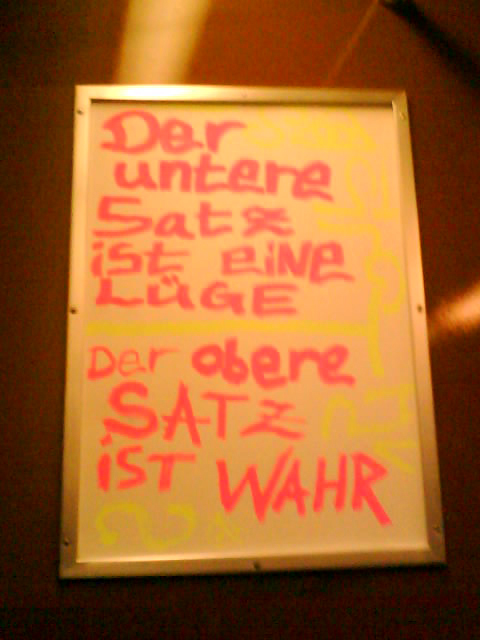
\includegraphics[scale=0.3]{material/13Pragv}
%%
%%\end{figure}
%
%\end{frame}


%%%%%%%%%%%%%%%%%%%%%%%%%%%%%%%%%%%%%%%
%%%%%%%%%%%%%%%%%%%%%%%%%%%%%%%%%%%%%%%
%
\subsubsection{Präsupposition}
%
%%%%%%%%%%%%%%%%%%%%%%%%%%%%%%%%%%%%%%%
%\iftoggle{sectoc}{
%	\begin{frame
%		\frametitle{~}
%		\tableofcontents[currentsubsection,subsubsectionstyle=hide]
%	}
%}
%%%%%%%%%%%%%%%%%%%%%%%%%%%%%%%%%%%%%%%

\begin{frame}
\frametitle{Präsupposition}

\begin{itemize}
	\item Implizite Voraussetzung ($\gg$)
	\item Präsuppositionen werden nicht vom Wahrheitsgehalt eines Satzes erfasst.
	\item Präsuppositionen müssen erfüllt sein, damit der Satz einen Wahrheitswert haben kann!

\vspace{1ex}

		\ea \label{ex11} Die aktuelle Präsidentin der USA ist erkältet.
		\z
		
		\begin{itemize}
			\item (\ref{ex11}) ist wahr, wenn es eine erkältete Präsidentin der USA gibt.
			\item (\ref{ex11}) ist falsch, wenn es keine erkältete Präsidentin der USA gibt.
			\item (\ref{ex11}) kann kein Wahrheitswert zugeordnet werden, wenn \gqq{es keine Präsidentin der USA gibt}.
		\end{itemize}
	
\end{itemize}

\end{frame}



%%%%%%%%%%%%%%%%%%%%%%%%%%%%%%%%%%%%%%%%%%%%%%%%%%%%%%%%%%%%%%%%

\begin{frame}
\frametitle{Präsupposition}

\begin{itemize}
	\item \textbf{Semantische} Präsupposition  (Bedingung für Wahrheit)
		
		p präsupponiert semantisch q, gdw.

		\begin{itemize}
			\item in allen Welten, in denen p wahr ist, auch q wahr ist,
			\item in allen Welten, in denen p falsch ist, q wahr ist.
			
			\ea Lauras Freundin ist blond. \hfill 
			\prspp\ Laura hat eine Freundin.
			\z
			
			\ea Lauras Freundin ist nicht blond. \hfill 
			\prspp\ Laura hat eine Freundin.
			\z
			
		\end{itemize}
	
	\item \textbf{Pragmatische} Präsupposition (Sprachgebrauch)

		Ein Sprecher S präsupponiert (pragmatisch) q mit der Äu\ss{}erung von p, wenn er davon ausgeht, dass q gemeinsames Sprecher-Hörer-Wissen ist.
			
		\ea A: Wer ist das Kind da drüben? \\
			   B: Der Sohn der Frau. \\
			   \ent\ A und B kennen \gqq{die Frau} und können daher die Phrase ohne Einführung verwenden.
		\z
	
\end{itemize}

\end{frame}


%%%%%%%%%%%%%%%%%%%%%%%%%%%%%%%%%%%%%%%%%%%%%%%%%%%%%%%%%%%%%%%%%%%

\begin{frame}
\frametitle{Präsuppositionstests}

\begin{itemize}
	\item Zur Unterscheidung von Präsuppositionen und Assertionen (wahrheitsfunktionaler Gehalt einer Äu\ss{}erung)
	\medskip
	\item \textbf{Negationstest}
	
	\begin{itemize}
		\item Präsupposition bleibt erhalten (vgl. semantische Implikation)		
		
		\ea Maria hat aufgehört zu rauchen.\\ $\gg$ Maria hat geraucht.
		\z
		
		\ea Es ist nicht der Fall, dass Maria aufgehört hat zu rauchen.\\ $\gg$ Maria hat geraucht.
		\z
		
	\end{itemize}	

\end{itemize}	



\end{frame}


%%%%%%%%%%%%%%%%%%%%%%%%%%%%%%%%%%%%%%%

\begin{frame}
\frametitle{Präsuppositionstests}

\begin{itemize}
	\item \textbf{Modalisierungstest}
	
	\begin{itemize}
		\item Präsupposition bleibt erhalten (vgl. semantische Implikation)

		\ea Peters Freundin ist krank.\\ $\gg$ Peter hat eine Freundin.
		\z
		
		\ea Peters Freundin ist wahrscheinlich/vielleicht krank.\\ $\gg$ Peter hat eine Freundin.
		\z
	
	\end{itemize}
	
\end{itemize}

\end{frame}


%%%%%%%%%%%%%%%%%%%%%%%%%%%%%%%%%%%%%%%%%%%%%%%%%%%%

\begin{frame}
\frametitle{Präsuppositionstest}

\begin{itemize}
	\item \textbf{Frage- und Aufforderungstest}
	
	\begin{itemize}
		\item Präsupposition bleibt erhalten (vgl. semantische Implikation)
		
		\ea Peter geht immer noch zum Sport.\\ \prspp\ Peter ging zum Sport.
		\z
		
		\ea Geht Peter immer noch zum Sport?\\ \prspp\ Peter ging zum Sport.
		\z
		
		\ea Geh (immer noch) zum Sport!\\ \prspp\ Peter ging zum Sport.
		\z
		
		
%		\ea Peter schlägt immer noch seine Frau.\\ $\gg$ Peter hat seine Frau geschlagen.
%		\z
%		
%		\ea Schlägt Peter immer noch seine Frau?\\ $\gg$ Peter hat seine Frau geschlagen.
%		\z
%		
%		\ea Schlag (immer) noch deine Frau!\\ $\gg$ Peter hat seine Frau geschlagen.
%		\z
		
		\end{itemize}

\end{itemize}

\end{frame}


%%%%%%%%%%%%%%%%%%%%%%%%%%%%%%%%%%%%%%% 

\begin{frame}
\frametitle{Präsuppositionstests}

\begin{itemize}
\item \textbf{Konditionalisierungstest}

\vspace{5mm}

	\begin{itemize}
		\item Präsupposition bleibt erhalten (vgl. semantische Implikation)
		
		\ea Auch Andrea spielt Tennis.\\ \prspp\ Eine weitere Person spielt Tennis.
		\z
		
		\ea Wenn auch Andrea Tennis spielt, hat sie dieses Wochenende ein Tunier.\\ \prspp\ Eine weitere Person spielt Tennis.
		\z
		
%		\ea Auch Andrea studiert noch.\\
%			$\gg$ Andrea studierte bisher.\\
%			$\gg$ Andere studieren auch.
%		\z
%
%			\ea Wenn auch Andrea noch studiert, dann bekommt sie kein Bafög mehr. \\
%			$\gg$ Andrea studierte bisher.\\
%			$\gg$ Andere studieren auch.
%		\z

	\end{itemize}
	
\end{itemize}

\end{frame}


%%%%%%%%%%%%%%%%%%%%%%%%%%%%%%%%%%%%%%%%%%%%%%%

%\begin{frame}
%\frametitle{Präsuppositionstests}
%
%\begin{itemize}
%	\item Präsuppositionen werden nicht durch Wahrheitsbedingungen erfasst.
%	
%	\begin{itemize}
%		\item negierbar, erfragbar, modalisierbar
%	\end{itemize}
%	
%	\item Präsupposition muss erfüllt sein, damit der Satz einen Wahrheitswert haben kann!
%	
%	\ea \label{ex21} Der gegenwärtige König von Frankreich ist kahlköpfig.
%	\z
%		
%		\begin{itemize}
%			\item (\ref{ex21}) ist wahr, wenn es einen König von Frankreich gibt, der kahlköpfig ist.
%			\item (\ref{ex21}) ist falsch, wenn es einen König von Frankreich gibt, der aber nicht kahlköpfig ist.
%			\item (\ref{ex21}) kann kein Wahrheitswert zugeordnet werden, wenn \gqq{es keinen König von Frankreich gibt}!
%		\end{itemize}
%
%\end{itemize}
%
%\end{frame}


%%%%%%%%%%%%%%%%%%%%%%%%%%%%%%%%%%%%%%%%%%%%%%%

\begin{frame}
\frametitle{Präsuppositionsauslöser}

\begin{itemize}
	\item \textbf{Eigennamen \& Definite DPs} (\zB \MyPobj{Jakob}, \MyPobj{der Präsident, der Tisch}, usw.)
	
	\ea Jakob isst gerne Pasta. \\ $\gg$ Es gibt ein Individuum namens Jakob.
	\z
	
	\ea Der Präsident von Amerika trägt einen Anzug.\\ $\gg$ Es gibt (genau) einen Präsident von Amerika.
	\z
	

%	\item \textbf{Definite DPs}
%	
%	\ea Der König von Frankreich ist kahlköpfig.\\ 
%	$\gg$ Es gibt (genau) einen König von Frankreich.
%	\z
	
	\item \textbf{Verben der Zustandsveränderung} (\zB \MyPobj{aufhören, anfangen}, usw.)

	\ea Es hat begonnen zu regnen.\\
			$\gg$ Es hat (davor) nicht geregnet.
	\z
	
	\item \textbf{Gradpartikeln} (\zB \MyPobj{nur, auch, sogar}, usw.)
	
	\ea Nur Luise ist weggefahren. \\
			$\gg$ Luise ist weggefahren.
	\z		

\end{itemize}

\end{frame}


%%%%%%%%%%%%%%%%%%%%%%%%%%%%%%%%%%%%%%%%%%%%%%%

\begin{frame}
\frametitle{Präsuppositionsauslöser}

\begin{itemize}
	\item \textbf{Temporalsätze} (\zB \MyPobj{bevor} \dots, \MyPobj{nachdem} \dots, \MyPobj{während} \dots, usw.)
	
	\ea Bevor Sie die Klausur geschrieben haben, hatten Sie Ihre Hausaufgaben zurückbekommen. \\ $\gg$ Sie haben die Klausur geschrieben.
	\z
	
	\item \textbf{Temporaladverbien} (\zB \MyPobj{noch, immer noch}, usw.)
	
	\ea Peter ist noch krank.\\ $\gg$ Peter war krank.
	\z
	
	\item \textbf{Faktive Verben} (\zB \MyPobj{wissen, vergessen dass, bedauern}, usw.)
	
	\ea Sie wissen, dass Sie abgehört werden.\\ $\gg$ Sie werden abgehört.
	\z

\end{itemize}

\end{frame}
%%%%%%%%%%%%%%%%%%%%%%%%%%%%%%%%%%%%%%%%%%%%%%%

%\begin{frame}
%\frametitle{Präsuppositionsaufhebung}
%
%\begin{itemize}
%	\item Aufhebbarkeit durch
%	
%\vspace{5mm}
%
%	\begin{itemize}
%		\item unmittelbaren Kontext:
%		
%		\ea Maria hat Peter nicht verlassen.\\
%			$\gg$ Maria war mit Peter zusammen.
%		\z
%		
%		\item Maria hat Peter nicht verlassen, denn sie waren nie zusammen.
%		
%\vspace{5mm}
%
%		\item Diskurskontext:
%		
%		\ea Peter bedauert, den Wagen gekauft zu haben.\\ 
%			$\gg$ Peter hat den Wagen gekauft.
%		\z
%			
%		\item Peter wird nicht bedauern (müssen), den Wagen gekauft zu haben \\(auch möglich, wenn Peter den Wagen nicht gekauft hat).
%				
%	\end{itemize}
%					
%\end{itemize}
%
%
%\end{frame}


%%%%%%%%%%%%%%%%%%%%%%%%%%%%%%%%%%%%%%%%%%%%%%%
%
\subsubsection{Implikatur}
%
%%%%%%%%%%%%%%%%%%%%%%%%%%%%%%%%%%%%%%%%%%%%%%%
%\iftoggle{sectoc}{
%	\begin{frame
%		\frametitle{~}
%		\tableofcontents[currentsubsection,subsubsectionstyle=hide]
%	}
%}
%%%%%%%%%%%%%%%%%%%%%%%%%%%%%%%%%%%%%%%%%%%%%%%


\begin{frame}
\frametitle{Implikatur}

\begin{itemize}
	\item vom englischen Philosophen \citet{Grice89a} geprägter Terminus
	\medskip
\begin{block}{Implikaturen}
	Bedeutungsaspekte einer Äu\ss{}erung, die nicht explizit erwähnt wurden. Sie sind nicht durch die Wahrheitsbedingungen eines Satzes erfassbar.
\end{block}	
%	\item Implikaturen:\\


	\begin{itemize}
		\item explizit Gesagtes \ras semantisch beschreibbar
		\item nicht explizit Gesagtes \ras implikatiert
	\end{itemize}


	\item Implikation \ras implizieren/folgern
	\item Implikatur \ras implikatieren
	\medskip
	\item konventionelle Implikaturen (umstritten)
	\item konversationelle Implikaturen
\end{itemize}

\end{frame}


%%%%%%%%%%%%%%%%%%%%%%%%%%%%%%%%%%%%%%%%%%%%%%%

\begin{frame}
\frametitle{Konventionelle Implikatur}

\begin{itemize}
	\item konventionelle Implikaturen: umstritten
	\medskip
	\item \textbf{konventionell} \ras mit der (konventionellen) Bedeutung eines Ausdrucks verbunden
	\medskip
	\item keinen Einfluss auf die Wahrheitsbedingung des Satzes
	
	\begin{itemize}
	\item Die konventionelle Implikatur gehört zu einem Ausdruck dazu, bestimmt aber nicht die Bedingungen, unter denen er wahr ist.
	\end{itemize}
	
\end{itemize}

\end{frame}


%%%%%%%%%%%%%%%%%%%%%%%%%%%%%%%%%%%%%%%%%%%%%%%

\begin{frame}
\frametitle{Konventionelle Implikatur}

\begin{columns}
\begin{column}[t]{0.6\textwidth}
	\begin{itemize}
		
		\item \textit{und} vs. \textit{aber}:
		
		\begin{itemize}
			\item gleiche Wahrheitsbedingungen
			\item \textit{aber}: Kontrast zu einer Erwartung
		\end{itemize}
	
		\eal 
		\ex Maria ist Italienerin aber liebt spanischen Wein.
		\ex Maria ist Italienerin und liebt spanischen Wein.
		\zl
	
		\item \textit{sogar}:
		
		\begin{itemize}
			\item Überraschung
		\end{itemize}
	
		\eal 
		\ex Sogar Jakob hat die Klausur bestanden.	
		\ex Jakob hat die Klausur bestanden.
		\zl
	
	\end{itemize}
	
\end{column}
\begin{column}[t]{0.4\textwidth}
	
\begin{itemize}

	\item \textit{du} vs. \textit{Sie}:
	
	\begin{itemize}
		\item gleiche Wahrheitsbedingungen
		\item soziale Distanz zwischen Sprecher und Hörer
	\end{itemize}

		\eal
		\ex Du bist Professor.
		\ex Sie sind Professor.
		\zl
	
\end{itemize}

\end{column}
\end{columns}


%
%	\eal 
%	\ex Maria ist schwanger aber fährt Fahrrad.
%	\ex Maria ist schwanger und fährt Fahrrad.
%	\zl
%
%\begin{itemize}	
%	\item \textit{und} vs. \textit{aber}:
%		
%	\begin{itemize}
%		\item Gleiche Wahrheitsbedingungen
%		\item \textit{aber} \ras Kontrast zu einer Erwartung
%	\end{itemize}
%
%
%	\eal 
%	\ex Sogar Maria hat die Klausur bestanden.	
%	\ex Maria hat die Klausur bestanden.
%	\zl
%
%	\item \textit{sogar}:
%		
%	\begin{itemize}
%		\item Überraschung
%	\end{itemize}
%
%	\eal
%	\ex Du bist Professor.
%	\ex Sie sind Professor.
%	\zl
%	
%	\item \textit{du} vs. \textit{Sie}:
%	
%	\begin{itemize}
%		\item gleiche Wahrheitsbedingungen
%		\item soziale Distanz zwischen Sprecher und Hörer
%	\end{itemize}
%		
%\end{itemize}

\end{frame}


%%%%%%%%%%%%%%%%%%%%%%%%%%%%%%%%%%%%%%%%%%%%%%%

%\begin{frame}
%\frametitle{Konventionelle Implikatur}
%
%\begin{itemize}
%	\item Du bist Professor. vs. Sie sind Professor.
%	
%	\begin{itemize}
%		\item \textit{du} vs. \textit{Sie}:
%		
%		\begin{itemize}
%			\item Gleiche Wahrheitsbedingung
%			\item \gqq{Gesellschaftliches Gefälle}
%		\end{itemize}
%		
%	\end{itemize}
%	
%	\item Nicht aufhebbar \ras ohne sich selbst zu widersprechen
%	\medskip
%	\item Ablösbar/abtrennbar
%	
%	\eal
%	\ex Sogar Maria ist schwanger.
%	\ex Maria ist schwanger.
%	\zl
%	
%	\end{itemize}
%
%\end{frame}


%%%%%%%%%%%%%%%%%%%%%%%%%%%%%%%%%%%%%%%%%%%%%%%

\begin{frame}
\frametitle{Konversationelle Implikatur}

\begin{itemize}
	\item konventionelle Implikatur: per Konvention mit einem Ausdruck verbunden
	\medskip
	\item konversationelle Implikatur (\implc ):
Folgerungen, die nur in bestimmten Äu\ss{}erungssituationen (d.\,h. in Abhängigkeit vom Kontext) entstehen

\vspace{5mm}

	\begin{itemize}
		\item Kontext: Nach einem Fussballspiel
		
		\ea A: Wie hat dir das Spiel gefallen?\\ B: Also, das Wetter war sehr gut!\\
		\item[] \implc Das Spiel hat B nicht gefallen.
		\z
	\end{itemize}
	
\end{itemize}

\end{frame}


%%%%%%%%%%%%%%%%%%%%%%%%%%%%%%%%%%%%%%%%%%%%%%%

\begin{frame}
\frametitle{Konversationelle Implikatur}

\begin{itemize}
	\item Basis für konversationelle Implikatur: Kooperationsprinzip
	\medskip
	\item Sprecher und Hörer befolgen (\idR) das Kooperationsprinzip.
	\item Das Kooperationsprinzip steuert die Konversation.
	
	\medskip
	
	\begin{block}{Kooperationsprinzip}
		Gestalte deinen Beitrag zur Konversation so, wie es dem Zweck und der Richtung des Gesprächs angemessen ist.
		
		\begin{itemize}
			\item Maxime der Qualität
			\item Maxime der Quantität
			\item Maxime der Relevanz
			\item Maxime der Modalität
		\end{itemize}
	
	\end{block}
	
\end{itemize}

\end{frame}


%%%%%%%%%%%%%%%%%%%%%%%%%%%%%%%%%%%%%%%%%%%%%%%

\begin{frame}
\frametitle{Konversationelle Implikatur}

\begin{block}{Maxime der Qualität}
	Versuche deinen Beitrag so zu gestalten, dass er wahr ist (sage nichts, was du für falsch hältst oder wofür du keine Anhaltspunkte hast).
	
	\ea A: Klaus hat einen Masterabschluss.\\
			\implc A ist sich sicher, dass Klaus einen Masterabschluss hat.
	\z
\end{block}

\begin{block}{Maxime der Quantität}
	Gestalte deinen Beitrag so informativ wie erforderlich (nicht mehr und nicht weniger Information als nötig).
	
	\ea Die Tasche ist schwarz.\\
			\implc Die Tasche ist vollständig schwarz.
	\z
\end{block}

\end{frame}

%%%%%%%%%%%%%%%%%%%%%%%%%%%%%%%%%%%%%%%%%%%%%%%
\begin{frame}
\frametitle{Konversationelle Implikatur}

\begin{block}{Maxime der Relevanz}
	Sage nur Relevantes.
	
	\ea A: Ich habe Hunger.\\
		   B: Ich kenne einen guten neuen Laden.\\
		   \implc In diesem Laden kann A etwas zum Essen kaufen.
	\z
\end{block}

\begin{block}{Maxime der Modalität}
	Rede klar und unzweideutig, kurz und bündig, geordnet.
	
	\ea Der blaue kuboide Block steht auf der Pyramide.\\
		   \implc Der blaue Block ist kein Würfel.
	\z
\end{block}

\end{frame}


%%%%%%%%%%%%%%%%%%%%%%%%%%%%%%%%%%%%%%%%%%%%%%%

\begin{frame}
\frametitle{Konversationelle Implikatur}

\begin{itemize}
	\item Konversationelle Implikaturen
	
\vspace{5mm}
	
	\begin{itemize}
		\item Durch Befolgung von Maximen
		\medskip
		\item Durch scheinbare Verletzung von Maximen
		\medskip
		\item Durch offensichtliche Hinwegsetzung über eine Maxime
	\end{itemize}
	
\end{itemize}

\end{frame}



%%%%%%%%%%%%%%%%%%%%%%%%%%%%%%%%%%%%%%%

\begin{frame}
\frametitle{Konversationelle Implikatur}

\begin{itemize}

	\item Verletzung der Qualitätsmaxime (Ironie)

	\ea Syntax war heute mal wieder spannend!\\
	\implc Syntax war langweilig.
	\z

\medskip

	\item Verletzung der Qualitätsmaxime (Ironie)
	
	\item[] \textbf{Kontext A}: Es regnet.
	
	\ea Schönes Wetter heute.\\
	\implc Das Wetter ist scheu\ss{}lich.
	\z
	
\medskip	
	
	\item (scheinbare) Verletzung der Relevanzmaxime
	
	\item[] \textbf{Kontext B}: Peter redet laut über Frau Müller, sieht aber nicht, dass diese hinter ihm steht. In dieser Situation äu\ss{}ert Maria den Satz:
	
	\ea Schönes Wetter heute.\\
	\implc Wechsle schnell das Thema! 
	\z	
		
	\end{itemize}

\end{frame}


%%%%%%%%%%%%%%%%%%%%%%%%%%%%%%%%%%%%%%%

\begin{frame}
\frametitle{Konversationelle Implikatur}

\begin{itemize}

	\item Befolgung der Quantitätsmaxime

	\ea Einige Schüler haben die Hausaufgabe gemacht.\\
	\implc nicht alle Schüler haben die Hausaufgabe gemacht.
	\z
	
\medskip
	
	\item Verletzung der Quantitäts- und/oder Relevanzmaxime
	
	\item[] \textbf{Kontext}: Empfehlungsschreiben für einen Kandidaten für einen Lehrstuhl der Philosophie

	\ea Sehr geehrte Damen und Herren, Herr X spricht ein gutes Deutsch, seine Handschrift ist leserlich und sein Besuch der Übungen war regelmä\ss{}ig. Mit freundlichen Grü\ss{}en \dots \\
	\implc Herr X eignet sich nicht für diese Position.
	\z
	
\end{itemize}

\end{frame}


%%%%%%%%%%%%%%%%%%%%%%%%%%%%%%%%%%%%%%%

\begin{frame}
\frametitle{Konversationelle Implikatur}

\begin{itemize}
	
	\item Verletzung der Maxime der Modalität (Fasse dich kurz!)
	
	\ea Gehen Sie zur Tür, drücken Sie den Griff im Uhrzeigersinn so weit hinunter wie möglich und ziehen Sie die Tür dann zu sich heran. \\
	\implc Verwenden Sie besondere Sorgfalt darauf, die Tür zu öffnen!\\
	\implc Ihnen beschreib ich's lieber ganz genau, bevor Sie wieder was falsch machen. (Spott)
	\z

\medskip
	
	\item Befolgung der Modalitätsmaxime
	
	\ea Karo ging in den Laden und kaufte sich eine Hose.\\
	\implc Karo ging zuerst in den Laden und kaufte dort eine Hose.
	\z
	
\end{itemize}

\end{frame}


%%%%%%%%%%%%%%%%%%%%%%%%%%%%%%%%%%%%%%%

%\begin{frame}
%\frametitle{Konversationelle Implikatur}
%
%\begin{itemize}
%	\item Konversationelle Implikaturen sind aufhebbar (vgl. konventionelle Implikatur).
%	
%		\ea Einige sind zur Klausur zugelassen. Sogar alle sind zur Klausur zugelassen!
%		\z
%	
%	\item Konversationelle Implikaturen sind nicht durch eine Paraphrase ablösbar (vgl. konventionelle Implikatur).
%	
%	\ea Peter trifft eine Frau.\\
%	\implc Peter trifft sich nicht mit seiner Frau.\\
%Peter begegnet einem Menschen weiblichen Geschlechts.
%	\z
%	
%\end{itemize}
%
%\end{frame}


%%%%%%%%%%%%%%%%%%%%%%%%%%%%%%%%%%%%%%% 

\begin{frame}
\frametitle{Konversationelle Implikatur}

\begin{figure}
\centering

%\begin{minipage}[t]{0.45\textwidth}
%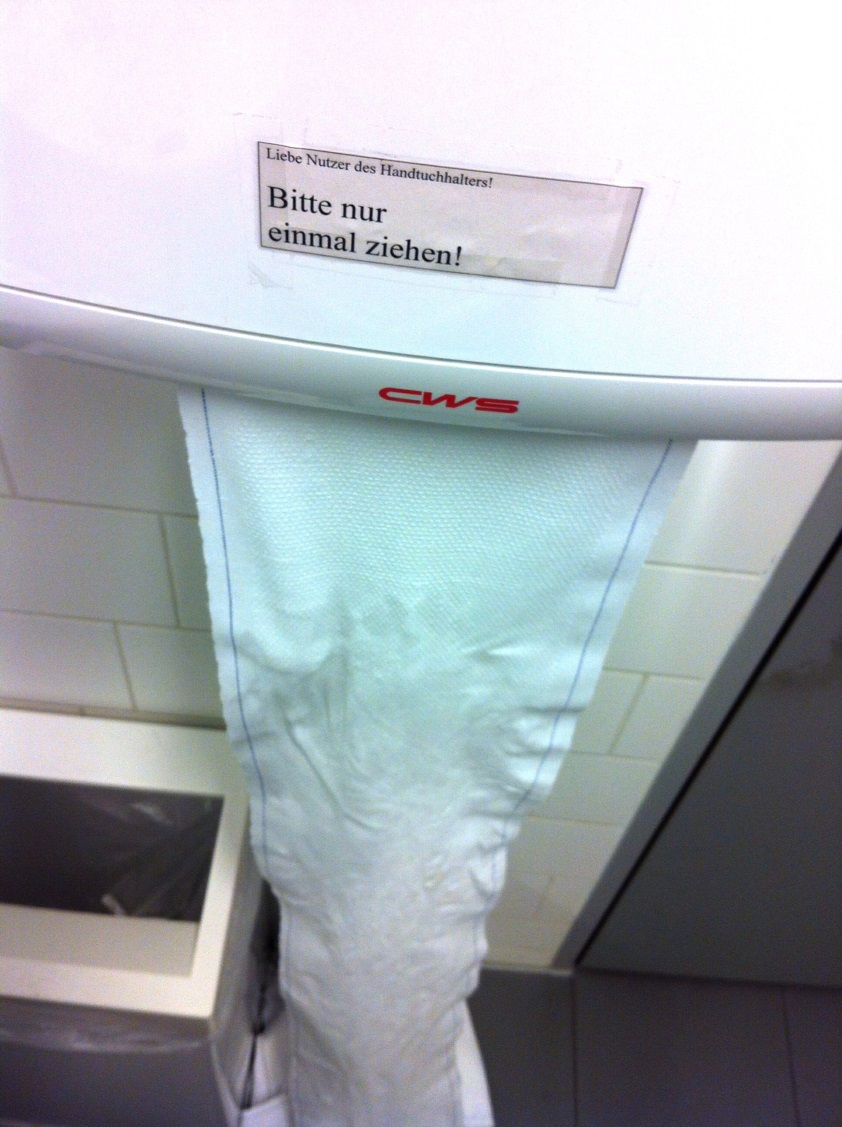
\includegraphics[width=\textwidth]{material/14Prag2}
%\end{minipage}
%
\begin{minipage}[t]{0.40\textwidth}
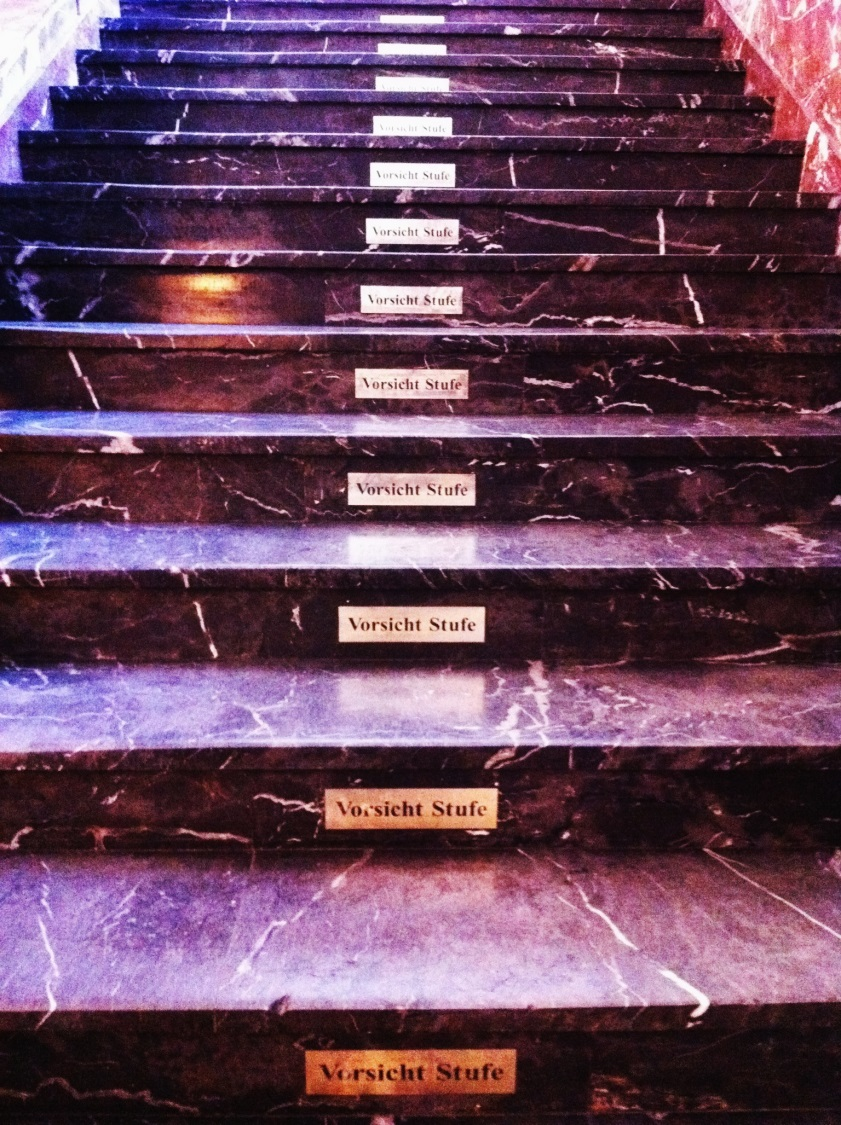
\includegraphics[width=\textwidth]{material/15Prag3}
\end{minipage}

\end{figure}

\end{frame}

%%%%%%%%%%%%%%%%%%%%%%%%%%%%%%%%%%%%%%%%%%%
\subsection{Übungen}
%%%%%%%%%%%%%%%%%%%%%%%%%%%%%%%%%%%%%%%%%%%
%% MyP: Contents
\iftoggle{sectoc}{
	\frame{
		%\begin{multicols}{2}
		\frametitle{~}
		\tableofcontents[currentsubsection,subsubsectionstyle=hide]
		%\end{multicols}
	}
}
%%%%%%%%%%%%%%%%%%%%%%%%%%%%%%%%%%%%%%%%%%%

\begin{frame}
%	[shrink]
\frametitle{Übungen}

	\begin{enumerate}
		\item Gegeben sei der Satz unter (\ref{ex:08ue1}):
		
			\ea\label{ex:08ue1}
			Einige der US-amerikanischen Beamten wissen, wer Richard erdrosselt hat.
			\z
			
			Geben Sie bei jedem der Sätze unter (\ref{ex:08ue2})--(\ref{ex:08ue5}) an, ob es sich um eine Implikatur, oder ob es sich um eine Präsupposition zu (\ref{ex:08ue1}) handelt. Schreiben Sie die richtige Antwort hinter den jeweiligen Satz. Wenn es sich um eine Präsupposition handelt, testen Sie dies anhand eines der Präsuppositionstests. \\
		\textbf{NB:} Vorsicht, zuweilen wird keine der Relationen wiedergegeben!
		\ea 
		\ea\label{ex:08ue2} Es existieren US-amerikanische Beamte.
		\ex\label{ex:08ue3} Richard war ein Semantiker.
		\ex\label{ex:08ue4} Nicht alle US"=amerikanischen Beamten wissen, wer den Mord begangen hat.
		\ex\label{ex:08ue5} Richard wurde erdrosselt.
		\z	
		\z 
	\end{enumerate}

\end{frame}

%%%%%%%%%%%%%%%%%%%%%%%%%%%%%%%%%%%%%%%%%%%

\begin{frame}
	\begin{enumerate}
		\item[2.] Bestimmen und kennzeichnen Sie zwei deiktische Ausdrücke im Satz (\ref{ex:08ue6}). Geben Sie zudem eine Anapher mit ihrem Antezendens an.
		\ea\label{ex:08ue6} Angelika hat gestern erwähnt, dass Irene sich dort mit den Formeln amüsiert hat.
		\z 
		\item[3.] Kreuzen Sie für Satz (\ref{ex:08ue7}) alle Sätze in der unten stehenden Liste an, die (konversationelle) Implikaturen dieses Satzes darstellen.
		\ea \label{ex:08ue7} Gottfried hat einige Nachbarn beleidigt.
		\z 
		\begin{itemize}
			\item[$\circ$] Gottfried hat einen Nachbarn.
			\item[$\circ$] Gottfried hat nicht alle Nachbarn beleidigt.
			\item[$\circ$] Gottfried ist ein unbeliebter Mensch.
			\item[$\circ$] Gottfried hat etwas Unhöfliches gesagt.
			\item[$\circ$] Gottfried hat einige Nachbarn nicht beleidigt.
		\end{itemize}
	\end{enumerate}
\end{frame}

%%%%%%%%%%%%%%%%%%%%%%%%%%%%%%%%%%%%%%%

\iftoggle{ue-loesung}{
	
	%%%%%%%%%%%%%%%%%%%%%%%%%%%%%%%%%%
%% UE 2 - 08 Pragmatik
%%%%%%%%%%%%%%%%%%%%%%%%%%%%%%%%%%

\begin{frame}
\frametitle{Übung -- Lösung}
	
	\begin{enumerate}
		\item Gegeben sei der Satz unter (\ref{ex:08ue1}):
		
	\begin{exe}
		\exr{ex:08ue1} Einige der US-amerikanischen Beamten wissen, wer Richard erdrosselt hat.
	\end{exe}

		\item [] Geben Sie bei jedem der Sätze unter (\ref{ex:08ue2})--(\ref{ex:08ue5}) an, ob es sich um eine Implikatur, oder ob es sich um eine Präsupposition zu (\ref{ex:08ue1}) handelt. Schreiben Sie die richtige Antwort hinter den jeweiligen Satz. Wenn es sich um eine Präsupposition handelt, testen Sie dies anhand eines der Präsuppositionstests. \\
		\textbf{NB:} Vorsicht, zuweilen wird keine der Relationen wiedergegeben!
	\begin{exe}
		\exr{ex:08ue2} Es existieren US-amerikanische Beamte. \alertgreen{\ras Präsupposition}
		\exr{ex:08ue3} Richard war ein Semantiker. \alertgreen{\ras keine Relation}
		\exr{ex:08ue4} Nicht alle US"=amerikanischen Beamten wissen, wer den Mord begangen hat. \alertgreen{\ras Implikatur}
		\exr{ex:08ue5} Richard wurde erdrosselt. \alertgreen{\ras Präsupposition}
	\end{exe}

	\end{enumerate}
	
\end{frame}

%%%%%%%%%%%%%%%%%%%%%%%%%%%%%%%%%%%%%%%%%%%

\begin{frame}
	\frametitle{Übung -- Lösung}
	
	\begin{enumerate}
		\item[2.] Bestimmen und kennzeichnen Sie zwei deiktische Ausdrücke im Satz (\ref{ex:08ue6}). Geben Sie zudem eine Anapher mit ihrem Antezendens an.
	
	\begin{exe}
		\exr{ex:08ue6} Angelika hat gestern erwähnt, dass Irene sich dort mit den Formeln amüsiert hat.
	\end{exe}
		
		\begin{itemize}
			\item[] \alertgreen{Ausdruck: \emph{gestern}, Art: Temporaldeixis}
			\item[] \alertgreen{Ausdruck: \emph{dort}, Art: Lokaldeixis}
			\item[] \alertgreen{Anapher: \emph{sich}, Antezedens: \emph{Irene}}
			\item[] \alertgreen{Auch möglich: \emph{den Formeln} \ras Objektdeixis}
		\end{itemize}
		
	\end{enumerate}
	
\end{frame}

%%%%%%%%%%%%%%%%%%%%%%%%%%%%%%%%%%%%%%%%%%%%

\begin{frame}
	\frametitle{Übung -- Lösung}
	
	\begin{enumerate}
		\item[3.] Kreuzen Sie für Satz (\ref{ex:08ue7}) alle Sätze in der unten stehenden Liste an, die (konversationelle) Implikaturen dieses Satzes darstellen.
		
	\begin{exe}
		\exr{ex:08ue7} Gottfried hat einige Nachbarn beleidigt.
	\end{exe}

		\begin{itemize}
			\item[$\circ$] Gottfried hat einen Nachbarn.
			\item[\alertgreen{$\checkmark$}] \alertgreen{Gottfried hat nicht alle Nachbarn beleidigt.}
			\item[$\circ$] Gottfried ist ein unbeliebter Mensch.
			\item[\alertgreen{$\checkmark$}] \alertgreen{Gottfried hat etwas Unhöfliches gesagt.}
			\item[\alertgreen{$\checkmark$}] \alertgreen{Gottfried hat einige Nachbarn nicht beleidigt.}
		\end{itemize}
		
	\end{enumerate}


\end{frame}
	
}

%%%%%%%%%%%%%%%%%%%%%%%%%%%%%%%%%%%%%%%


	
	%% -*- coding:utf-8 -*-

%%%%%%%%%%%%%%%%%%%%%%%%%%%%%%%%%%%%%%%%%%%%%%%%%%%%%%%%%


\def\insertsectionhead{\refname}
\def\insertsubsectionhead{}

\huberlinjustbarfootline


\ifpdf
\else
\ifxetex
\else
\let\url=\burl
\fi
\fi
\begin{multicols}{2}
{\tiny
%\beamertemplatearticlebibitems

\bibliography{gkbib,bib-abbr,biblio}
\bibliographystyle{unified}
}
\end{multicols}





%% \section{Literatur}
%% \begin{frame}[allowframebreaks]
%% \frametitle{Literatur}
%% 	\footnotesize

%% \bibliographystyle{unified}

%% 	%German
%% %	\bibliographystyle{deChicagoMyP}

%% %	%English
%% %	\bibliographystyle{chicago} 

%% 	\bibliography{gkbib,bib-abbr,biblio}
	
%% \end{frame}

	
\end{document}


